\section{A known-answer study}
\label{sec:known}

Before the checks are trusted on real data, they are run where the answer is
known. Following Ismail et al.~\cite{ismail2020} and Tonekaboni et
al.~\cite{tonekaboni2020}, who test time-series explanations on generated data
with known important inputs, we generate weekly store data in which the effect
of every part of the plan is set by us, fit correct models and models with
failures planted on purpose, and ask two questions: which checks catch which
failure, and do the explanations of models that pass the checks match the
truth?

\subsection{Design}

\paragraph{The data}
Three price zones of six stores sell 20 items for 260 weeks
(Figure~\ref{fig:knownseries}). Expected sales are the item's size and season
times an unobserved demand shock (a first-order autoregression on the log
scale, standard deviation 0.25, persistence 0.7), times the effects in
Table~\ref{tab:knowntruth}. A temporary cut and a change in the regular price
have different elasticities, $-2.5$ and $-0.5$, as in the literature on
promotions and the Dominick's experiments. Each item gets one chain-wide
regular price rise of 3\% to 8\%. In each zone one store's regular prices rise
10\% and one store's fall 10\% for 16 weeks at random times during training,
and one rises and one falls starting at the forecast origin, week 253, so that
every model can be scored on them exactly as on Dominick's. Sales are Poisson
around their expectation.

\paragraph{Two worlds}
In the first, cuts, promotions and displays are planned at random. In the
second, merchants plan them more often in weeks when the unobserved demand
shock is high (the log odds of each rise by the shock in standard deviations),
as merchants do when they promote into strong weeks. Everything else is the
same.

\paragraph{The models}
In each world: the world model with three seeds; the world model fitted with
each series' prices shuffled across its training weeks, so that it cannot learn
a price effect (\emph{blind to price}); the world model fitted with promotion
and display shuffled the same way (\emph{blind to levers}); LightGBM; and
LightGBM blind to price. The forecast for weeks 253 to 260 is explained and
every check run as on real data; the world model has the settings of the
companion paper's Dominick's world model except that it is a single fit rather
than an average of three, without store switching, with width 32 and 2,000
steps, to fit on a processor; LightGBM has the companion paper's Dominick's
settings. Each explanation is also scored against the truth, computed from the
expected sales under the same counterfactual plans: rank agreement and the
ratio of summed lifts on the \kaPlanned{} of \kaRows{} item-weeks with
something planned, overall and by lever.

\begin{table}[t]
\centering
\caption{\textbf{The generated data have known effects for every part of the
plan.}}
\label{tab:knowntruth}
\footnotesize
\begin{tabular}{@{}lr@{}}
\toprule
Effect on expected sales & Size\\
\midrule
Temporary cut, elasticity on price over regular & $-2.5$\\
Regular price, elasticity on regular over list & $-0.5$\\
Promotion & $+40\%$\\
Display & $+25\%$\\
Promotion and display together, extra & $+15\%$\\
Week after a planned week with nothing planned & $-15\%$\\
\midrule
Chance of a cut; depth & 12\%; 10\% to 40\%\\
Chance of a promotion, with a cut; without & 60\%; 3\%\\
Chance of a display & 8\%\\
\bottomrule
\end{tabular}
\end{table}

\begin{figure}[t]
\centering
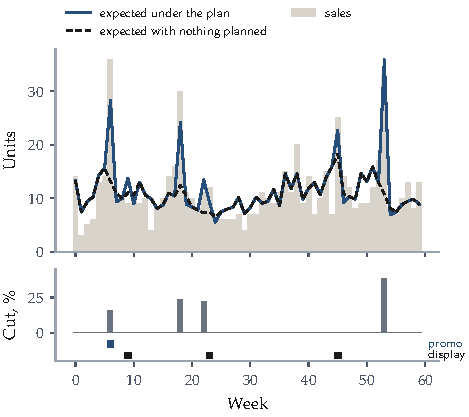
\includegraphics[width=\columnwidth]{figs/fig_known_series.pdf}
\caption{\textbf{In the generated data the effect of every part of the plan is
known.} One item in one store over 60 weeks, in the world where merchants plan
into high-demand weeks: sales, expected sales under the plan, and expected
sales with nothing planned; below, the cut and the weeks with a promotion or a
display.}
\label{fig:knownseries}
\end{figure}

\subsection{What the checks catch}

\begin{figure*}[t]
\centering
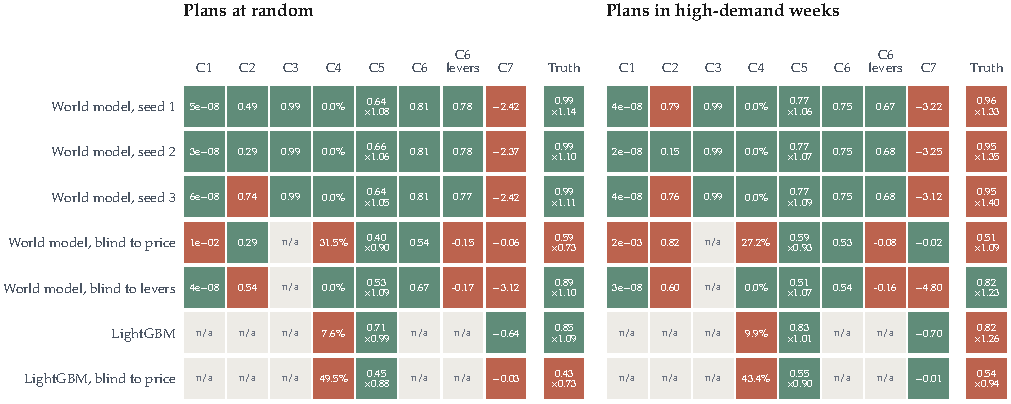
\includegraphics[width=\textwidth]{figs/fig_known_checks.pdf}
\caption{\textbf{Correct models pass the checks; so do models whose
explanations are wrong in ways only some checks can see.} Each check's score
and its pass (green) or fail (red) under the rules fixed in advance, for every
model in both worlds; grey, does not apply. C5: rank of predicted with observed
lift, and summed forecast over summed sales. C6 levers: the lowest per-lever
rank agreement with LightGBM, reported but without a rule fixed in advance.
C7: pooled slope of the stated response to the price spells at the origin,
passed when inside the 95\% interval of the measured slope. Truth: rank
agreement of the model's lifts with the true lifts and the ratio of their sums,
green when the rank is at least 0.7 and the ratio within 0.8 to 1.25.}
\label{fig:knownchecks}
\end{figure*}

\begin{figure*}[t]
\centering
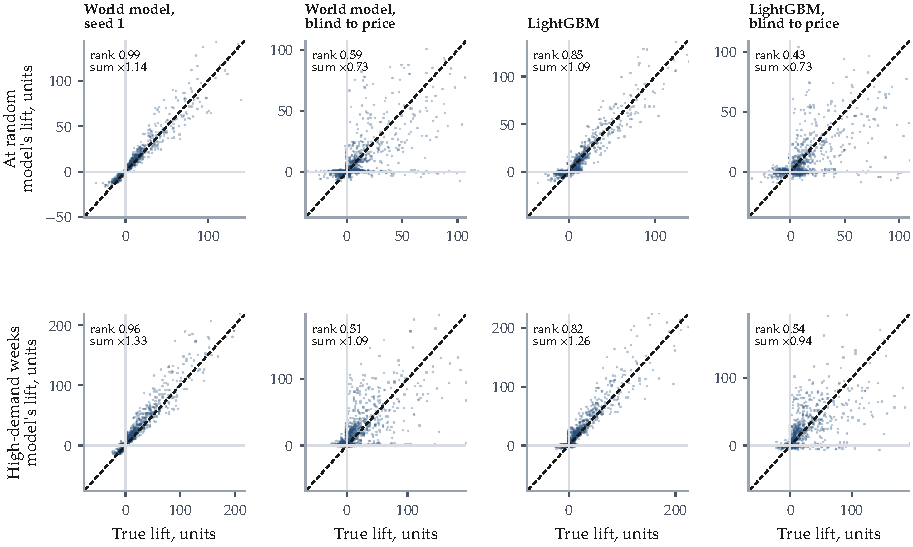
\includegraphics[width=\textwidth]{figs/fig_known_scatter.pdf}
\caption{\textbf{When plans follow demand, both the world model and LightGBM
overstate what the plan adds, and agree with each other.} Each point is an
item-week with something planned: the model's total lift against the true lift,
units. Dashed: equal. Top, plans at random; bottom, plans made more often in
high-demand weeks.}
\label{fig:knownscatter}
\end{figure*}

Figure~\ref{fig:knownchecks} shows every check on every model, and
Table~\ref{tab:known} in the appendix every score. Six results stand out.

\paragraph{Correct models pass, and their explanations are right}
With plans at random, the three world-model seeds pass every check that applies
except C2 for one seed, and their lifts match the truth: rank agreement
\kaClWmTruth{} and summed lift \kaClWmBias{} times the true lift for seed 1,
with the price, promotion and display parts each within 13\% of the truth.
Seeds agree on their lifts as closely as on their forecasts (C3, \kaClSeedRank).
LightGBM's lifts rank \kaClLgbTruth{} with the truth at \kaClLgbBias{} times.

\paragraph{The price check catches a model blind to price; the check against
sales does not}
All four models fitted without a usable price fail C4: \kaClWmNpCfour\% and
\kaCoWmNpCfour\% of item-weeks for the world model, \kaClLgbNpCfour\% and
\kaCoLgbNpCfour\% for LightGBM, against 0\% for the world models fitted on real
prices. All four pass C5: their forecasts on planned weeks sum to 0.88 to 0.93
of sales, with rank agreement 0.40 to 0.59. Their explanations are wrong in a
way a merchant would act on: the price part is zero, and the promotion, which
usually comes with a cut, takes its place, at 1.95 to 2.37 times its true lift
across the four (Figure~\ref{fig:knownscatter}).
Both price-blind world models also fail C1 narrowly, because the audit takes the
regular price from the true history while these models learned it from a
shuffled one; that is a property of how the failure was planted, not a sign
that C1 detects it.

\paragraph{Only a per-lever comparison catches lifts given to the wrong lever}
The world model fitted without usable promotion and display flags passes C1,
C4 and C5, and its total lift agrees with LightGBM's (C6, \kaClNlCsix{} and
\kaCoNlCsix) and ranks \kaClWmNlTruth{} with the truth. Its explanation gives
the promotion \kaClWmNlPromoBias{} and the display \kaClWmNlDisplayBias{} times
their true lift, and the price \kaClWmNlPriceBias{} times. Every check on the
total lift except C2 passes it. Its per-lever agreement with LightGBM does not:
\kaClNlCsixPromo{} for the promotion and \kaClNlCsixDisplay{} for the display,
against \kaClWmCsixPromo{} for the correct world model.

\paragraph{When plans follow demand, every check passes and the lifts are a
third too large}
In the second world the three world-model seeds pass C1, C3, C4, C5 and C6, and
their forecasts are more accurate than in the first (item-by-store RMSSE
\kaCoWmRmsse{} against \kaClWmRmsse{}): a plan made in high-demand weeks tells
the model about the demand. Their lifts are \kaCoWmBiasLo{} to \kaCoWmBiasHi{}
times the true lift, and the display's \kaCoWmDispLo{} to \kaCoWmDispHi{} times.
C5 cannot see this: sales in planned weeks are high for the same reason, and
the forecasts sum to \kaCoWmCfive{} times them. C6 cannot see it either:
LightGBM, fitted to the same data, overstates by \kaCoLgbBias{} times, and the
two agree at \kaCoWmCsix. No check that compares the explanation with the
model, with the data or with another model fitted to the same data can find a
bias that the data themselves carry.

\paragraph{The world model treats a regular price change like a temporary cut}
For the price spells that start at the origin, the world model's stated
response is $\kaClWmCsevenSlope$ per unit of log price with plans at random
and $\kaCoWmCsevenSlope$ when plans follow demand, in every seed; the truth is
$-0.5$, and $-2.5$ is the temporary-cut elasticity
(Figure~\ref{fig:knownc7}). It has learned how sales answer a cut and applies
it to a change in the regular price. LightGBM, whose inputs include the item's recent prices, states $\kaClLgbCsevenSlope$ and $\kaCoLgbCsevenSlope$. The measured
response from difference in differences on the generated sales is
$\kaClMeasSlope$ ($\kaClMeasLo$ to $\kaClMeasHi$) and $\kaCoMeasSlope$
($\kaCoMeasLo$ to $\kaCoMeasHi$): imprecise with six spells and three or four
controls each, as on Dominick's, but enough to reject the world model's answer
in both worlds and not LightGBM's. Apart from C2 for one seed, C7 is the only
check the world model fails in the first world, and the only one that finds this
error.

\paragraph{Randomisation does not separate working models from broken ones}
After the lift readout is re-initialised, the rank agreement of the lifts with
the original is \kaLiftReadLo{} to \kaLiftReadHi{} across world models, and it
stays at \kaEncLo{} to \kaEncHi{} with every part re-initialised
(Figure~\ref{fig:knowncascade}). The construction itself ties the lifts to the
weeks with something planned and to the size of the item, so a network with
random weights still ranks them much as the trained one does. C2 fails correct
seeds and passes broken models; as specified, it does not test a lift built
into the model, and we do not use it as evidence below.

\begin{figure*}[t]
\centering
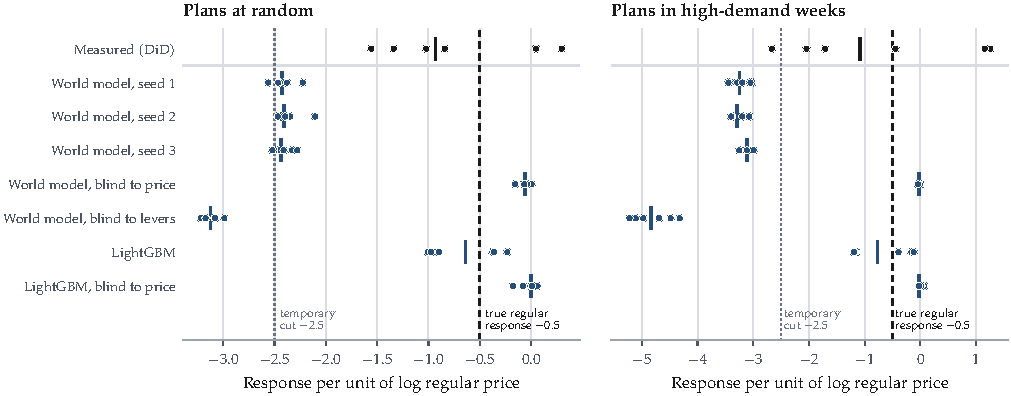
\includegraphics[width=\textwidth]{figs/fig_known_c7.pdf}
\caption{\textbf{Every world model states the response to a regular price
change as if it were a temporary cut; LightGBM does not.} The stated change in
store category units per unit of log price for each of the six price spells
that start at the forecast origin (dots; bar, median), against the measured
response from difference in differences on the generated sales (top row), the
true response ($-0.5$, dashed) and the temporary-cut elasticity ($-2.5$,
dotted).}
\label{fig:knownc7}
\end{figure*}

\begin{figure}[t]
\centering
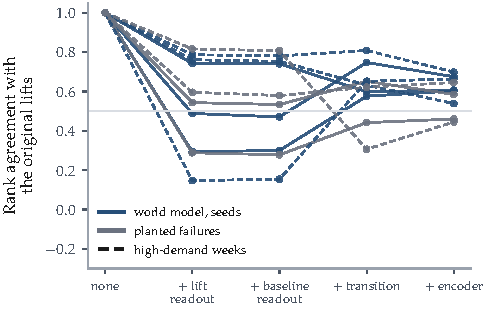
\includegraphics[width=\columnwidth]{figs/fig_known_cascade.pdf}
\caption{\textbf{Re-initialising the network leaves the lifts' ranking largely
in place.} C2 for every world model, both worlds: rank agreement of the total
lift with the original after the lift readout, then the baseline readout, the
transition and the encoder are re-initialised in turn.}
\label{fig:knowncascade}
\end{figure}

\paragraph{What the study says about the checks}
Across the 14 models, the share of checks passed tracks how well a model ranks
the true lifts (Spearman \kaPassTruthRho) but not how close its lifts are in
size (\kaPassBiasRho{} with the negative absolute log ratio): the models that
pass the most checks include the confounded ones whose lifts are a third too
large. Accuracy tracks the gross failures, the price-blind models being the
least accurate, and misses the subtle ones. The checks earn their place as
follows. C4 finds a model that ignores price. Per-lever agreement with another
model finds lifts given to the wrong lever. C1 and C3 confirm construction and
stability. C5 and C6 confirm agreement but cannot find a bias the data carry,
and C2 as specified finds nothing. Only a measured cause, C7, finds that a
model's stated response to a price change is wrong, and only one kind of
response, a sustained regular-price change, has a measured cause on public
retail data.
